\documentclass[border=10pt]{standalone}
\usepackage[T1]{fontenc}
\usepackage{tikz}
\usepackage{fontawesome5}
\usepackage{amsmath,amssymb}

\usetikzlibrary{calc, positioning, arrows.meta, shapes.geometric, fit, backgrounds}

% ── Modern Academic Conference Palette ──
\definecolor{colImgBg}{RGB}{245,247,250}
\definecolor{colImgBorder}{RGB}{180,192,205}
\definecolor{colColmapBg}{RGB}{240,247,255}
\definecolor{colColmapBorder}{RGB}{140,180,225}
\definecolor{colGSBg}{RGB}{254,244,236}
\definecolor{colGSBorder}{RGB}{245,155,100}
\definecolor{colWebBg}{RGB}{242,250,244}
\definecolor{colWebBorder}{RGB}{125,195,145}

\definecolor{colPrimary}{RGB}{45,95,165}
\definecolor{colAccent}{RGB}{235,95,45}
\definecolor{colGreen}{RGB}{50,150,85}
\definecolor{colText}{RGB}{35,45,60}
\definecolor{colSubText}{RGB}{100,115,130}
\definecolor{colArr}{RGB}{90,105,125}

\begin{document}
\sffamily
\begin{tikzpicture}[
    >=Latex,
    font=\sffamily,
    block/.style={
        rounded corners=8pt,
        line width=0.9pt,
        align=center,
        inner sep=8pt,
        text=colText
    },
    arr/.style={->, >=Latex, line width=1.15pt, color=colArr},
    arrDashed/.style={->, >=Latex, line width=1.0pt, dashed, color=colArr},
    lbl/.style={font=\sffamily\scriptsize\itshape, text=colSubText, fill=white, inner sep=1.5pt, rounded corners=2pt}
]

% ════════════════════════════════════════════
% STAGE 1: Monocular Video & Sharp Frames
% ════════════════════════════════════════════
\begin{scope}[shift={(0, -0.1)}]
    % Outer container block
    \draw[colImgBorder, fill=white, rounded corners=8pt, line width=0.9pt]
        (-1.25, -1.05) rectangle (1.25, 2.30);

    % Stage Title
    \node[font=\sffamily\bfseries\footnotesize, text=colText] at (0, 1.95)
        {Monocular Video};

    % Fan of frames inside block
    \begin{scope}[shift={(-0.6, 0.05)}]
        % Frame 3 (Back)
        \fill[colImgBg, draw=colImgBorder, rounded corners=2.5pt, line width=0.5pt]
            (0.32, 0.35) rectangle ++(1.15, 0.85);

        % Frame 2 (Middle)
        \fill[colImgBg, draw=colImgBorder, rounded corners=2.5pt, line width=0.5pt]
            (0.16, 0.18) rectangle ++(1.15, 0.85);

        % Frame 1 (Front - Sharp Keyframe)
        \fill[white, draw=colImgBorder!90!black, rounded corners=2.5pt, line width=0.7pt]
            (0, 0) rectangle ++(1.15, 0.85);
        \fill[colPrimary!20, rounded corners=1.5pt] (0.12, 0.12) rectangle (0.5, 0.52);
        \fill[colAccent!30, rounded corners=1.5pt] (0.6, 0.12) rectangle (1.02, 0.65);
        \draw[colText!25, line width=0.4pt] (0.12, 0.72) -- (1.02, 0.72);

        % Check badge on front frame
        \node[font=\fontsize{5}{6}\selectfont, text=colGreen] at (0.98, 0.72) {\faCheckCircle};
    \end{scope}

    % Sub-labels
    \node[below, font=\sffamily\bfseries\scriptsize, text=colText] at (0, -0.32)
        {Frame Extraction};
    \node[below, font=\sffamily\scriptsize, text=colSubText] at (0, -0.62)
        {Laplacian Blur Filter};

    \coordinate (videoOut) at (1.25, 0.68);
\end{scope}

% ════════════════════════════════════════════
% STAGE 2: COLMAP Structure-from-Motion
% ════════════════════════════════════════════
\begin{scope}[shift={(4.15, -0.1)}]
    % Outer container block
    \draw[colColmapBorder, fill=colColmapBg, rounded corners=8pt, line width=0.9pt]
        (-1.25, -1.05) rectangle (1.25, 2.30);

    % Stage Title
    \node[font=\sffamily\bfseries\footnotesize, text=colText] at (0, 1.95)
        {COLMAP SfM};

    % Mini Frustums (Camera Poses)
    \begin{scope}[shift={(-0.6, 0.94)}]
        \draw[colPrimary, line width=0.7pt, fill=colPrimary!15]
            (-0.2, 0.2) -- (0.2, 0.2) -- (0, -0.15) -- cycle;
        \draw[colPrimary!60, line width=0.5pt] (0, -0.15) -- (-0.1, 0.3);
    \end{scope}
    \begin{scope}[shift={(0.6, 0.94)}]
        \draw[colPrimary, line width=0.7pt, fill=colPrimary!15]
            (-0.2, 0.2) -- (0.2, 0.2) -- (0, -0.15) -- cycle;
        \draw[colPrimary!60, line width=0.5pt] (0, -0.15) -- (0.1, 0.3);
    \end{scope}

    % Feature rays intersecting
    \draw[colPrimary!40, dashed, line width=0.5pt] (-0.6, 0.79) -- (0, 0.26);
    \draw[colPrimary!40, dashed, line width=0.5pt] (0.6, 0.79) -- (0, 0.26);

    % Sparse 3D Point Cloud dots
    \foreach \pt in {(-0.4, 0.34), (-0.15, 0.48), (0.1, 0.29), (0.4, 0.38),
                     (-0.3, 0.11), (0.0, 0.14), (0.35, 0.01), (-0.15, -0.09), (0.2, -0.14)} {
        \fill[colAccent] \pt circle (1.4pt);
    }

    % Sub-labels
    \node[below, font=\sffamily\bfseries\scriptsize, text=colText] at (0, -0.32)
        {Pose Estimation};
    \node[below, font=\sffamily\scriptsize, text=colSubText] at (0, -0.62)
        {SIFT \& Sparse Cloud};

    \coordinate (colmapIn) at (-1.25, 0.68);
    \coordinate (colmapOutTop) at (1.25, 1.20);
    \coordinate (colmapOutBot) at (1.25, 0.18);
\end{scope}

% ════════════════════════════════════════════
% STAGE 3: 3D Gaussian Splatting (3DGS)
% ════════════════════════════════════════════
\begin{scope}[shift={(8.55, -0.1)}]
    % Outer container block
    \draw[colGSBorder, fill=colGSBg, rounded corners=8pt, line width=0.9pt]
        (-1.45, -1.05) rectangle (1.45, 2.30);

    % Stage Title
    \node[font=\sffamily\bfseries\footnotesize, text=colText] at (0, 1.95)
        {3DGS Optimization};

    % Densely packed anisotropic 3D Gaussians (ellipsoids)
    \begin{scope}[shift={(0, 0.70)}]
        \fill[colAccent, opacity=0.45] (-0.65, -0.25) ellipse [x radius=0.22, y radius=0.12, rotate=25];
        \fill[colAccent, opacity=0.60] (-0.20, -0.32) ellipse [x radius=0.18, y radius=0.22, rotate=-15];
        \fill[colAccent, opacity=0.75] (0.42, -0.20) ellipse [x radius=0.25, y radius=0.14, rotate=35];
        \fill[colAccent, opacity=0.85] (-0.50, 0.15) ellipse [x radius=0.20, y radius=0.15, rotate=-30];
        \fill[colAccent, opacity=0.95] (0.05, 0.08) ellipse [x radius=0.26, y radius=0.16, rotate=15];
        \fill[colAccent, opacity=0.70] (0.58, 0.10) ellipse [x radius=0.16, y radius=0.22, rotate=-25];
        \fill[colAccent, opacity=0.60] (-0.30, 0.40) ellipse [x radius=0.22, y radius=0.13, rotate=40];
        \fill[colAccent, opacity=0.75] (0.28, 0.38) ellipse [x radius=0.19, y radius=0.14, rotate=-10];
    \end{scope}

    % Sub-labels
    \node[below, font=\sffamily\bfseries\scriptsize, text=colText] at (0, -0.32)
        {Differentiable Rasterizer};
    \node[below, font=\sffamily\scriptsize, text=colSubText] at (0, -0.62)
        {Adaptive Density Control};

    \coordinate (gsInTop) at (-1.45, 1.20);
    \coordinate (gsInBot) at (-1.45, 0.18);
    \coordinate (gsOut) at (1.45, 0.68);
\end{scope}

% ════════════════════════════════════════════
% STAGE 4: Export & Web Viewer (Three.js / WebGL)
% ════════════════════════════════════════════
\begin{scope}[shift={(12.9, -0.1)}]
    % Outer container block (Browser Window)
    \draw[colWebBorder, fill=white, rounded corners=8pt, line width=0.9pt]
        (-1.3, -1.05) rectangle (1.3, 2.30);

    % Browser Top Bar
    \fill[colWebBg, rounded corners=7pt]
        (-1.28, 1.78) rectangle (1.28, 2.28);
    \fill[white] (-1.28, 1.78) rectangle (1.28, 1.90); % flatten bottom border of bar
    \draw[colWebBorder!70, line width=0.5pt] (-1.3, 1.78) -- (1.3, 1.78);

    % Browser Window Dots
    \fill[red!60] (-1.05, 2.04) circle (1.8pt);
    \fill[yellow!80!orange] (-0.85, 2.04) circle (1.8pt);
    \fill[green!70!black] (-0.65, 2.04) circle (1.8pt);

    % Web Title inside bar
    \node[font=\sffamily\fontsize{7}{8.5}\selectfont\bfseries, text=colText] at (0.35, 1.96)
        {Client Viewer};

    % Interactive 3D Canvas
    \begin{scope}[shift={(0, 0.70)}]
        % Viewport background
        \fill[colWebBg!60, rounded corners=4pt] (-1.05, -0.48) rectangle (1.05, 0.68);
        \draw[colWebBorder!50, line width=0.5pt, rounded corners=4pt] (-1.05, -0.48) rectangle (1.05, 0.68);

        % Rendered Splat cluster in viewport
        \fill[colAccent!80, opacity=0.85] (0.05, 0.05) ellipse [x radius=0.35, y radius=0.20, rotate=15];
        \fill[colPrimary!70, opacity=0.75] (-0.35, -0.10) ellipse [x radius=0.25, y radius=0.15, rotate=-20];
        \fill[colGreen!80, opacity=0.70] (0.35, 0.15) ellipse [x radius=0.22, y radius=0.18, rotate=30];

        % Orbit Navigation Gizmo
        \draw[colPrimary!80, -{Latex[length=2.5pt]}, line width=0.6pt]
            (-0.7, 0.38) arc (160:20:0.45 and 0.18);
        \node[font=\fontsize{5}{6}\selectfont, text=colPrimary!80] at (-0.75, 0.20) {\faSync};
    \end{scope}

    % Sub-labels
    \node[below, font=\sffamily\bfseries\scriptsize, text=colText] at (0, -0.32)
        {Interactive 3D Viewer};
    \node[below, font=\sffamily\scriptsize, text=colSubText] at (0, -0.62)
        {Three.js / WebGL ($\ge$60 FPS)};

    \coordinate (webIn) at (-1.3, 0.68);
\end{scope}

% ════════════════════════════════════════════
% PIPELINE ROUTING & CONNECTORS
% ════════════════════════════════════════════

% 1. Video Frames to COLMAP
\draw[arr] (videoOut) -- (colmapIn)
    node[lbl, midway, above=1pt] {sharp frames};

% 2. COLMAP to 3DGS (Dual outputs: Poses & Sparse Cloud)
\draw[arr] (colmapOutTop) -- (gsInTop)
    node[lbl, midway, above=1pt] {camera poses};

\draw[arr] (colmapOutBot) -- (gsInBot)
    node[lbl, midway, below=1pt] {sparse point cloud};

% 3. 3DGS to Web Viewer (Export .ply / compressed splat)
\draw[arr] (gsOut) -- (webIn)
    node[lbl, midway, above=1pt] {\texttt{.ply} / splat};

\end{tikzpicture}
\end{document}
